\documentclass[10pt,a4paper]{article}

\usepackage[utf8]{inputenc}
\usepackage[T1]{fontenc}
\usepackage[brazil]{babel}
\usepackage{lmodern}
\usepackage[dvipsnames]{xcolor}
\usepackage{graphicx}
\usepackage{amsmath}
\usepackage{textcomp}
\usepackage{booktabs}
\usepackage{array}
\usepackage{tabularx}
\usepackage[hidelinks]{hyperref}
\usepackage{enumitem}
\usepackage{tikz}
\usepackage{lastpage}

\setlength{\oddsidemargin}{-1.04cm}   % 1.5cm - 1in
\setlength{\evensidemargin}{-1.04cm}
\setlength{\topmargin}{-1.1cm}
\setlength{\headheight}{28pt}
\setlength{\headsep}{0.35cm}
\setlength{\textwidth}{18.0cm}        % 21cm - 1.5cm - 1.5cm
\setlength{\textheight}{25.2cm}
\setlength{\marginparwidth}{0pt}
\setlength{\parindent}{0pt}
\setlength{\parskip}{4pt}

\newcommand{\legend}[1]{\par\vspace{2pt}\footnotesize\color{steel}#1}

\definecolor{unbblue}{HTML}{00296B}
\definecolor{unbgreen}{HTML}{1B7A3D}
\definecolor{steel}{HTML}{4A4A4A}
\definecolor{lightgray}{HTML}{F2F2F2}
\definecolor{copperline}{HTML}{B87333}
\definecolor{alertred}{HTML}{C1121F}

\hypersetup{pdftitle={RessonadorQuadrado -- Datasheet de Projeto},
            pdfsubject={Datasheet técnico -- Ressoador em espiral quadrada, RO5880},
            pdfauthor={J. V. V. Faria, T. Ferreira -- UnB/ENE},
            pdfkeywords={ODMR, NV-, HFSS, RO5880, ressoador, datasheet}}

% Pagestyle manual (sem fancyhdr - kernel MiKTeX desta máquina e
% incompatível com os hooks da versão atual do fancyhdr, mesmo
% problema documentado no relatório principal para o pacote geometry)
\makeatletter
\def\ps@rqds{%
  \def\@oddhead{\parbox{\textwidth}{\footnotesize\color{steel}%
    RessoadorQuadrado --- Espiral Quadrada Acoplada em RO5880\hfill
    Doc.\ RQ--RO5880--2026~~Rev.\ A\\[1pt]
    \textcolor{unbblue}{\rule{\textwidth}{0.6pt}}}}
  \def\@evenhead{\@oddhead}
  \def\@oddfoot{\parbox{\textwidth}{%
    \textcolor{unbblue}{\rule{\textwidth}{0.4pt}}\\[2pt]
    \footnotesize\color{steel}%
    UnB -- ENE -- Dept.\ Eng.\ El\'etrica\hfill\thepage~/~\pageref{LastPage}\hfill
    Setembro/2026}}
  \def\@evenfoot{\@oddfoot}
}
\makeatother
\pagestyle{rqds}

% ---- caixa de titulo estilo datasheet comercial ----
\newcommand{\titleblock}{%
\noindent
\begin{tikzpicture}[remember picture, overlay]
\fill[unbblue] (current page.north west) rectangle ([yshift=-2.6cm]current page.north east);
\end{tikzpicture}
\vspace*{-1.05cm}
\noindent
\begin{minipage}[c]{0.22\textwidth}
  
\includegraphics[height=1.55cm]{../assets/unb_marca/as_bas_cor_jpg/as_bas_cor.jpg}
\end{minipage}%
\begin{minipage}[c]{0.56\textwidth}
  \centering
  \color{white}\Large\bfseries RessoadorQuadrado\\[2pt]
\end{minipage}%
\begin{minipage}[c]{0.22\textwidth}
  \centering
  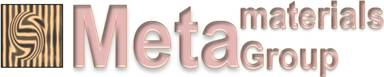
\includegraphics[height=1.15cm]{../assets/gmeta/gmeta_banner.jpg}
\end{minipage}
\vspace{0.15cm}

% ---- bloco de autores ----
\noindent
\begin{center}
\footnotesize\color{steel}
\textbf{Autores:} Jo\~ao Victor Vieira Faria \quad$\vert$\quad Thiago Ferreira\\[1pt]
Departamento de Engenharia El\'etrica (ENE) -- Universidade de Bras\'ilia (UnB)\\[1pt]
\textbf{Orientador:} Prof.\ Dr.\ Achiles Fontana da Mota
\end{center}
\vspace{0.15cm}
}

% ---- caixa cinza com borda para tabelas/paineis ----
\newenvironment{panel}[1]{%
  \par\noindent\textcolor{unbblue}{\rule{\textwidth}{1.1pt}}\\[1pt]
  {\bfseries\color{unbblue} #1}\\[2pt]
  \textcolor{unbblue}{\rule{\textwidth}{0.4pt}}\\[4pt]
}{%
  \par\vspace{2pt}
}

\begin{document}
\titleblock

\begin{minipage}[t]{0.47\textwidth}
\begin{panel}{CARACTER\'ISTICAS}
\begin{itemize}[leftmargin=14pt, itemsep=1pt, topsep=0pt]
  \item Ressonador de micro-ondas de \textbf{1 porta} (reflexão), topologia
        espiral quadrada com acoplamento por gap
  \item Frequência de projeto: \textbf{2,87\,GHz} (desdobramento de campo
        zero do centro NV$^-$ em diamante, para ODMR)
  \item Substrato \textbf{Rogers RT/duroid~5880}, $h=0{,}75$\,mm,
        $\varepsilon_r \approx 2{,}20$
  \item Metalização em cobre, $t=35\,\mu$m (1\,oz), face superior
        (traço) e plano de terra sólido na face inferior
  \item Footprint da placa: \textbf{55,0 $\times$ 50,0\,mm}
  \item Footprint do ressonador (espiral): \textbf{7,25 $\times$ 7,50\,mm}
  \item Simulado por elementos finitos no Ansys HFSS (driven modal,
        porta tipo \emph{Lumped Port}/rede terminal)
  \item Arquivos de fabricação (máscara 1:1, normal e espelhada) prontos
        para corrosão com percloreto/cloreto de ferro
\end{itemize}
\end{panel}
\end{minipage}%
\hfill
\begin{minipage}[t]{0.47\textwidth}
\begin{panel}{APLICA\c{C}\~AO}
Manipulação de spin de centros de vacância de nitrogênio (NV$^-$) em
diamante via resson\^ancia magn\'etica detectada opticamente (ODMR).
O ressonador gera o campo de micro-ondas necess\'ario para excitar a
transi\c{c}\~ao de desdobramento de campo zero (\emph{zero-field
splitting}) do NV$^-$, em 2,87\,GHz, concentrando o campo magn\'etico
RF pr\'oximo da amostra de diamante posicionada sobre a espiral.
\end{panel}
\begin{panel}{RESUMO DE DESEMPENHO (simulado)}
\begin{tabular}{@{}p{5.0cm}r@{}}
Frequ\^encia de melhor casamento $f_0$ & 2,885\,GHz \\
$S_{11}$ em $f_0$ & $-16{,}1$\,dB \\
$S_{11}$ em 2,87\,GHz (alvo) & $-1{,}22$\,dB \\
VSWR em 2,87\,GHz (alvo) & 14,2 \\
Desvio $f_0$ $\rightarrow$ alvo & $\approx$ 15\,MHz \\
\end{tabular}
\end{panel}
\end{minipage}

\vspace{4pt}
\begin{panel}{DESCRI\c{C}\~AO}
O RessoadorQuadrado \'e um ressonador planar de micro-ondas de porta \'unica,
formado por uma espiral quadrada de tr\^es voltas em cobre (objeto
\texttt{Square\_Spiral} no modelo HFSS), acoplada por proximidade
(\emph{gap coupling}, $g_{cpl}=0{,}5$\,mm) a uma linha de alimenta\c{c}\~ao
microstrip (\texttt{Feedline}) que se estende at\'e a borda da placa,
onde um conector coaxial (porta \texttt{Port\_Sheet}) excita o circuito.
O plano de terra \'e cobre s\'olido cont\'inuo na face inferior do
substrato -- n\~ao h\'a padr\~ao a corroer nessa camada. O par\^ametro
medido \'e $S_{11}=S(\mathrm{Port1},\mathrm{Port1})$; por ser porta \'unica,
n\~ao existe $S_{21}$.
\end{panel}

\clearpage

\begin{panel}{1. PAR\^AMETROS GEOM\'ETRICOS (variáveis de projeto no HFSS)}
\begin{center}
\renewcommand{\arraystretch}{1.15}
\begin{tabular}{lll}
\toprule
\textbf{Simbolo} & \textbf{Descrição} & \textbf{Valor} \\
\midrule
$L_{sub}$   & Lado X do substrato               & 55,0\,mm \\
$W_{sub}$   & Lado Y do substrato (medido)       & 50,0\,mm \\
$h_{sub}$   & Espessura do substrato             & 0,75\,mm \\
$t_{cu}$    & Espessura do cobre                 & 0,035\,mm (1\,oz) \\
$a_{spiral}$& Passo base da espiral (parâmetro)  & 3,5\,mm \\
$w_{spiral}$& Largura da trilha da espiral       & 0,5\,mm \\
$g_{spiral}$& Espaçamento entre voltas           & 0,5\,mm \\
$p_{spiral}$& Passo (pitch $=w+g$)               & 1,0\,mm \\
$z_{spiral}$& Deslocamento vertical/offset       & 0,7675\,mm \\
$w_{feed}$  & Largura da linha de alimentação    & 2,5\,mm \\
$g_{cpl}$   & Gap de acoplamento feed--espiral   & 0,5\,mm \\
$L_{cpl}$   & Comprimento de acoplamento         & 5,0\,mm \\
\bottomrule
\end{tabular}
\end{center}
\legend{Valores extraídos por leitura direta das \texttt{VariableProp} do
arquivo \texttt{RessoadorQuadrado.aedt} (projeto não alterado). Dimensões
de footprint medidas diretamente na geometria real (face de topo do
cobre) sao apresentadas na Se\c{c}\~ao~3.}
\end{panel}

\begin{panel}{2. MATERIAIS, PORTA E SETUP DE SOLUCAO}
\begin{center}
\renewcommand{\arraystretch}{1.15}
\begin{tabular}{lll}
\toprule
\textbf{Item} & \textbf{Especificação} & \textbf{Valor} \\
\midrule
Substrato & Material & Rogers RT/duroid 5880 (tm) \\
Condutor  & Material & Cobre (copper), $\sigma$ padrão da biblioteca HFSS \\
Região de fundo & Material & Vácuo (radiation boundary) \\
\midrule
Porta & Tipo & Lumped Port \\
Porta & Rede & HFSS Terminal Network \\
Porta & Quantidade & 1 (\texttt{Port1}) \\
\midrule
Solver & Tipo & HFSS Driven, solu\c{c}\~ao \emph{Single} \\
Solver & Motor linear & Direct Solver \\
Adaptativo & Frequ\^encia & 2,87\,GHz \\
Adaptativo & Crit\'erio & $\Delta S_{max}=0{,}02$, at\'e 15 passes \\
Varredura & Faixa & 2,0 -- 4,0\,GHz \\
Varredura & Resolu\c{c}\~ao & 401 pontos (LinearCount), tipo \emph{Fast} \\
\bottomrule
\end{tabular}
\end{center}
\legend{Extra\'ido por parsing de texto (\texttt{Setup1}/\texttt{Sweep}) do
arquivo \texttt{.aedt} -- o projeto nunca foi aberto/alterado para gerar
este datasheet.}
\end{panel}

\clearpage

\begin{panel}{3. VISTAS DA ESTRUTURA (3D e 2D, dimensoes reais)}

\begin{minipage}{0.48\textwidth}
\centering
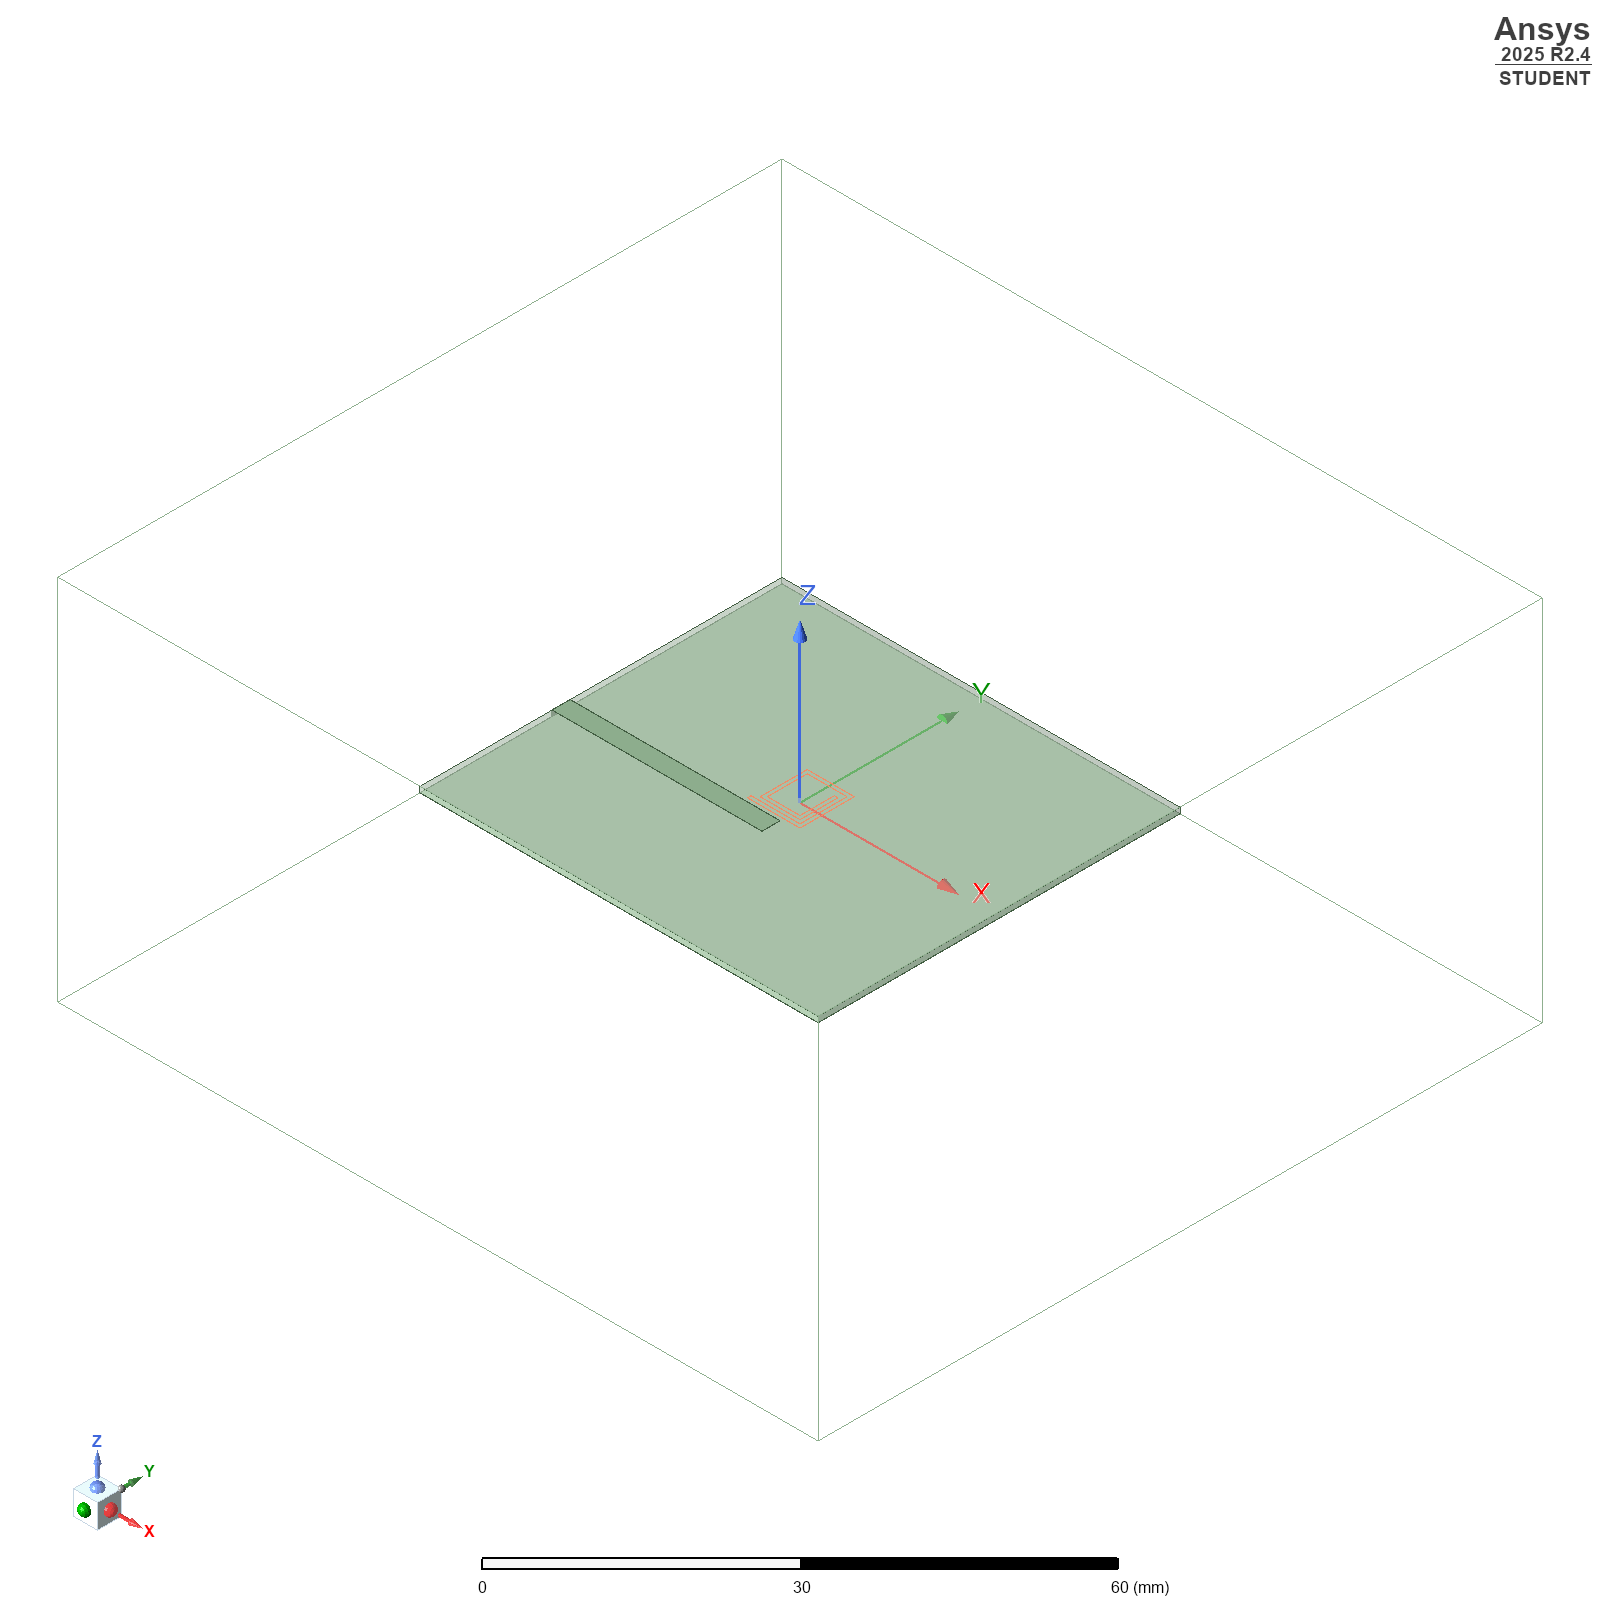
\includegraphics[width=\textwidth]{../../aedt_project/datasheet_figs/view_iso.png}\\[2pt]
\footnotesize Figura 1 -- Vista isométrica 3D do modelo completo (placa
55$\times$50\,mm), renderizada diretamente do HFSS.
\end{minipage}%
\hfill
\begin{minipage}{0.48\textwidth}
\centering
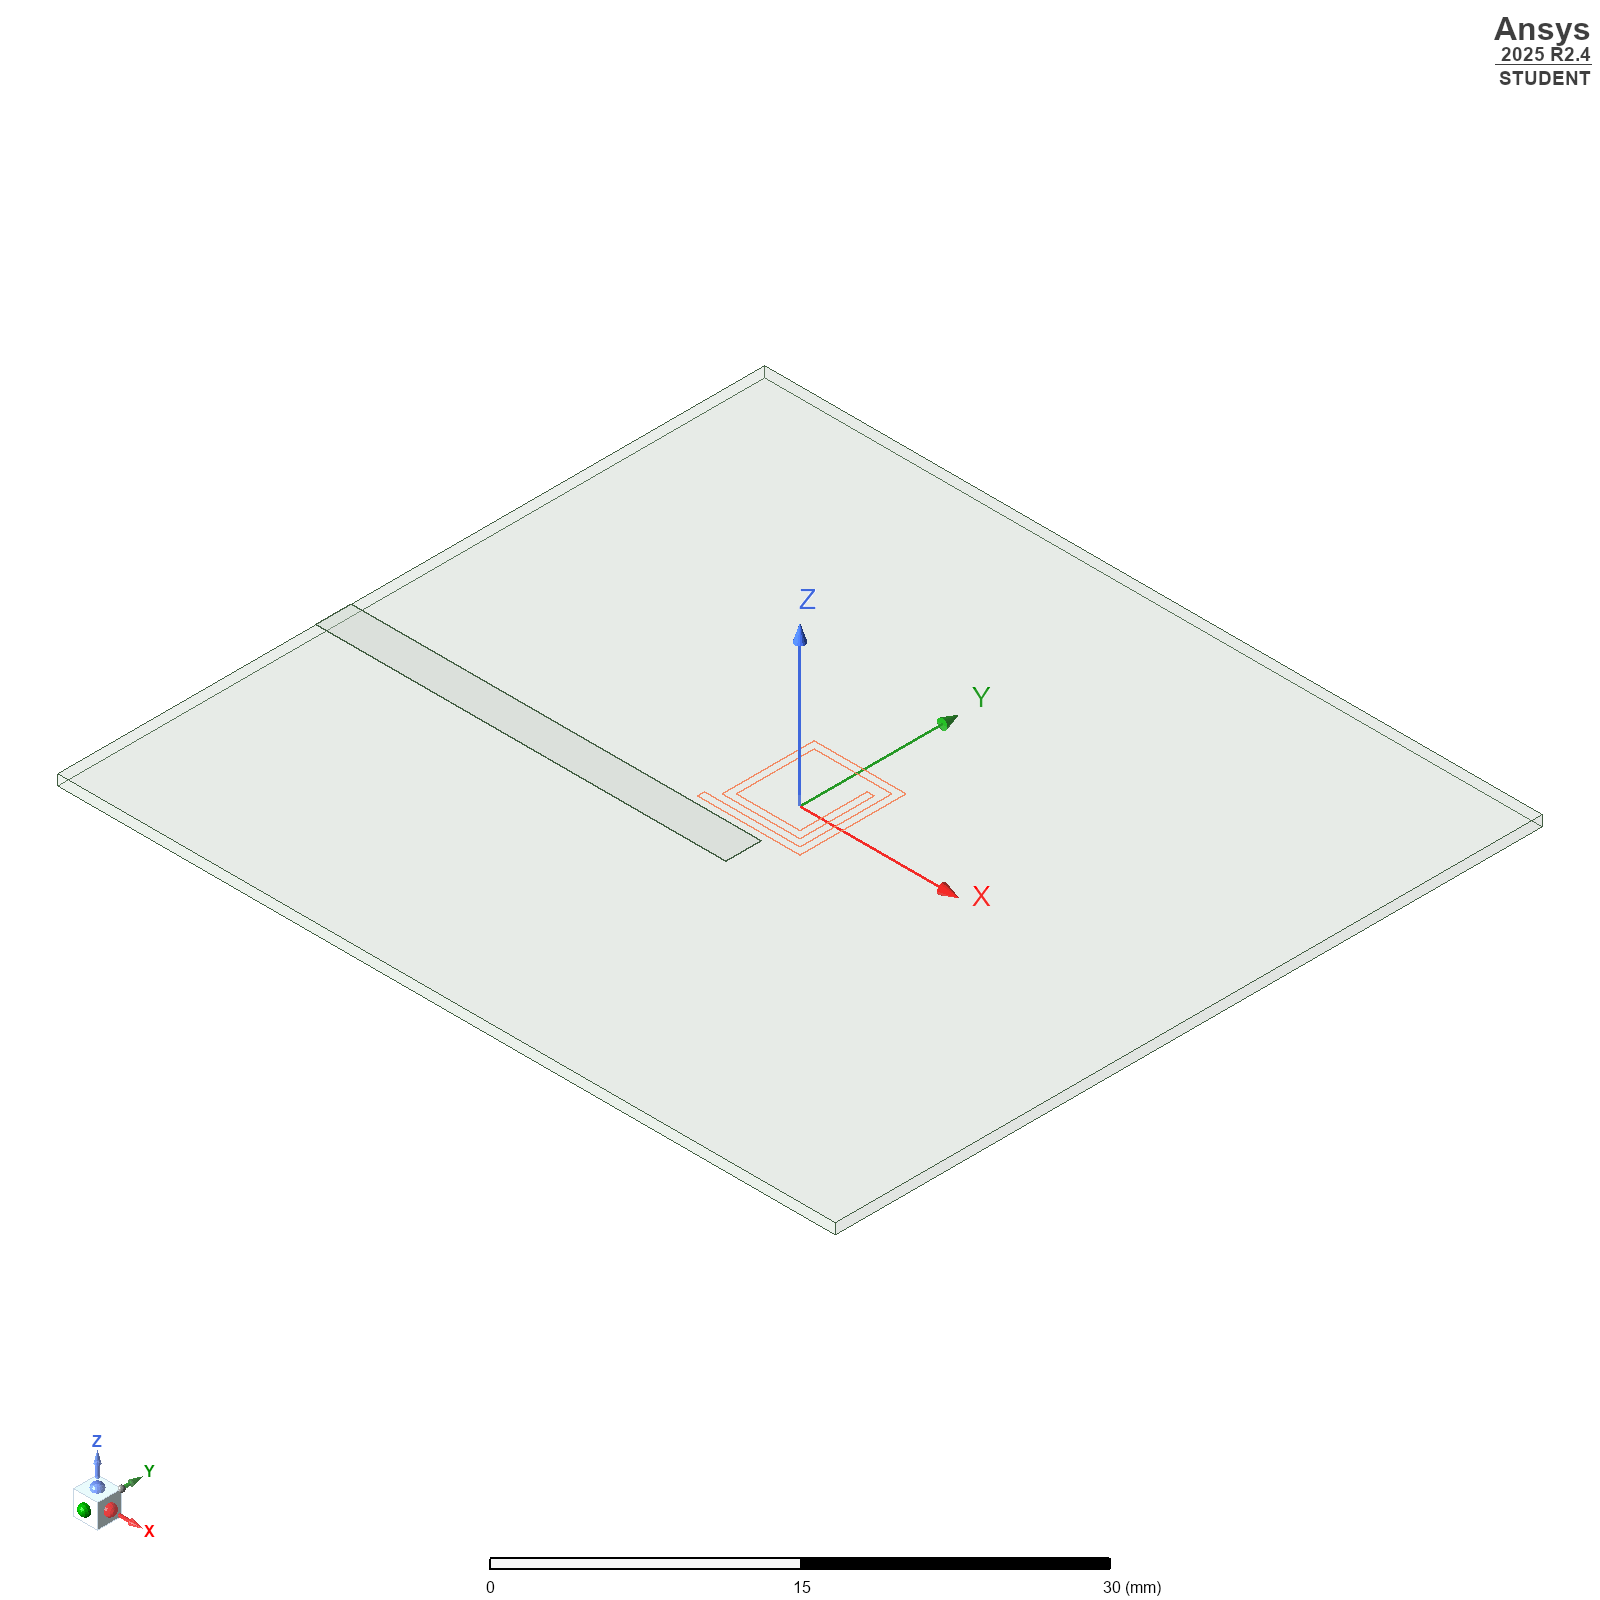
\includegraphics[width=\textwidth]{../../aedt_project/datasheet_figs/view_iso_zoom.png}\\[2pt]
\footnotesize Figura 2 -- Detalhe isométrico 3D da região do ressonador
(espiral + trilha de acoplamento).
\end{minipage}

\vspace{8pt}
\begin{center}
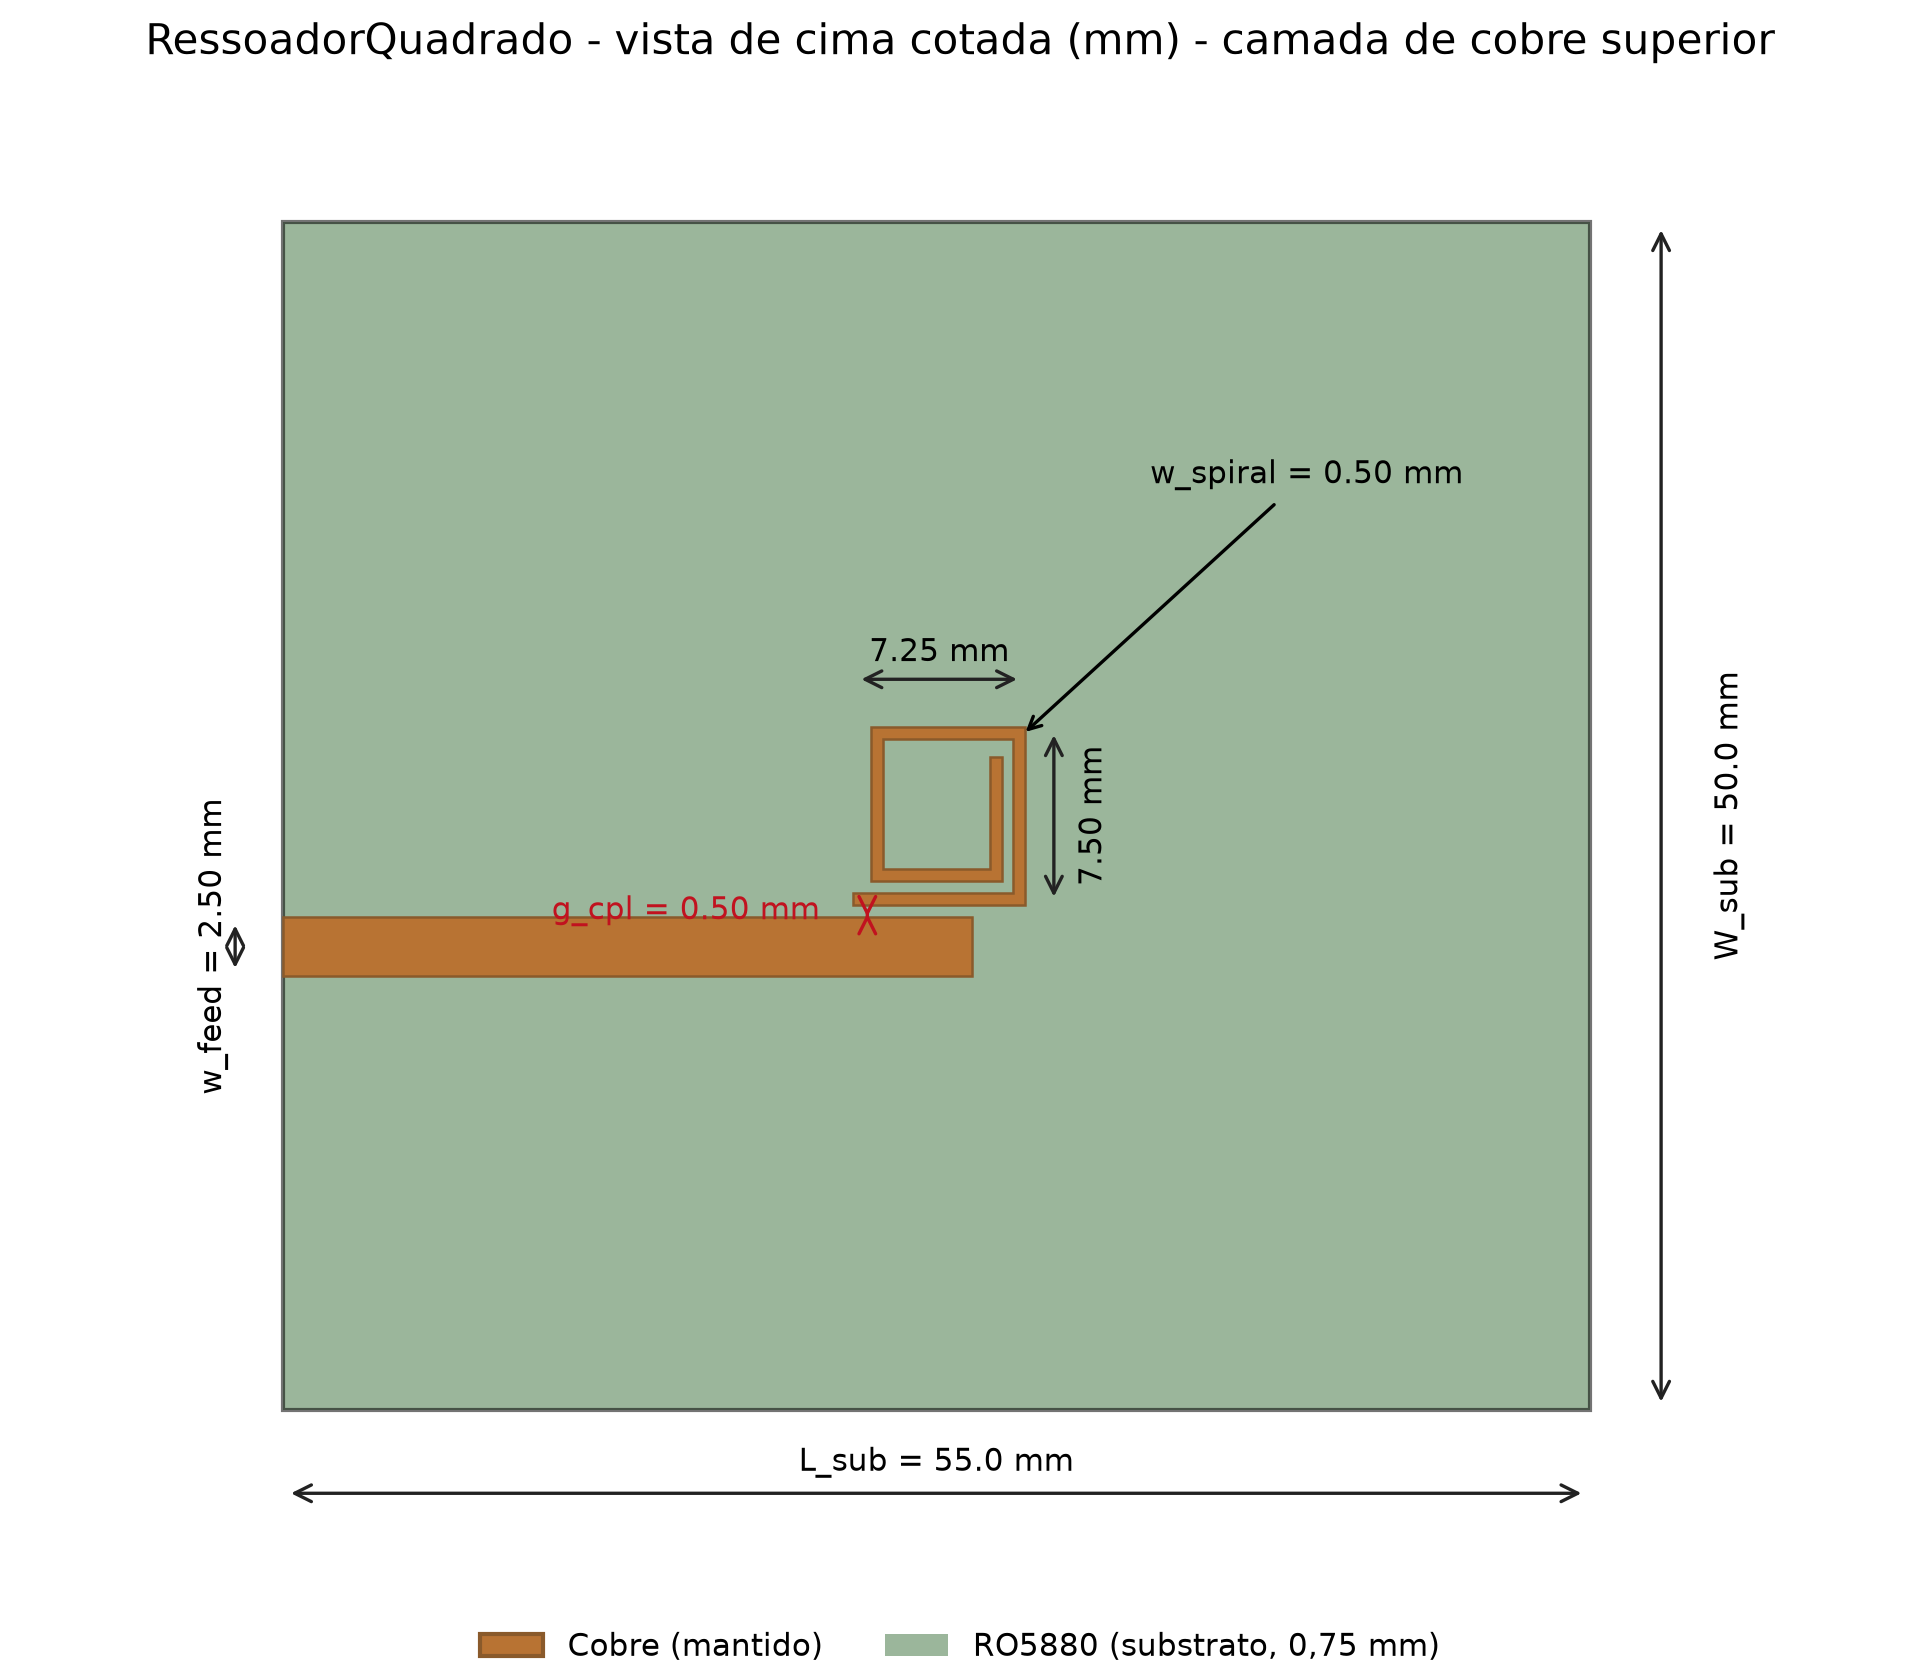
\includegraphics[width=0.72\textwidth]{../../aedt_project/datasheet_figs/fig_drawing_top.png}\\[2pt]
\footnotesize Figura 3 -- Desenho de engenharia cotado (vista de cima, camada
de cobre superior), com todas as cotas de fabricação em mm --
geometria extraida diretamente dos vértices reais do modelo HFSS
(não redesenhada manualmente).
\end{center}
\end{panel}

\clearpage

\begin{panel}{4. DESEMPENHO EL\'ETRICO T\'IPICO (simulado, HFSS)}
\begin{center}
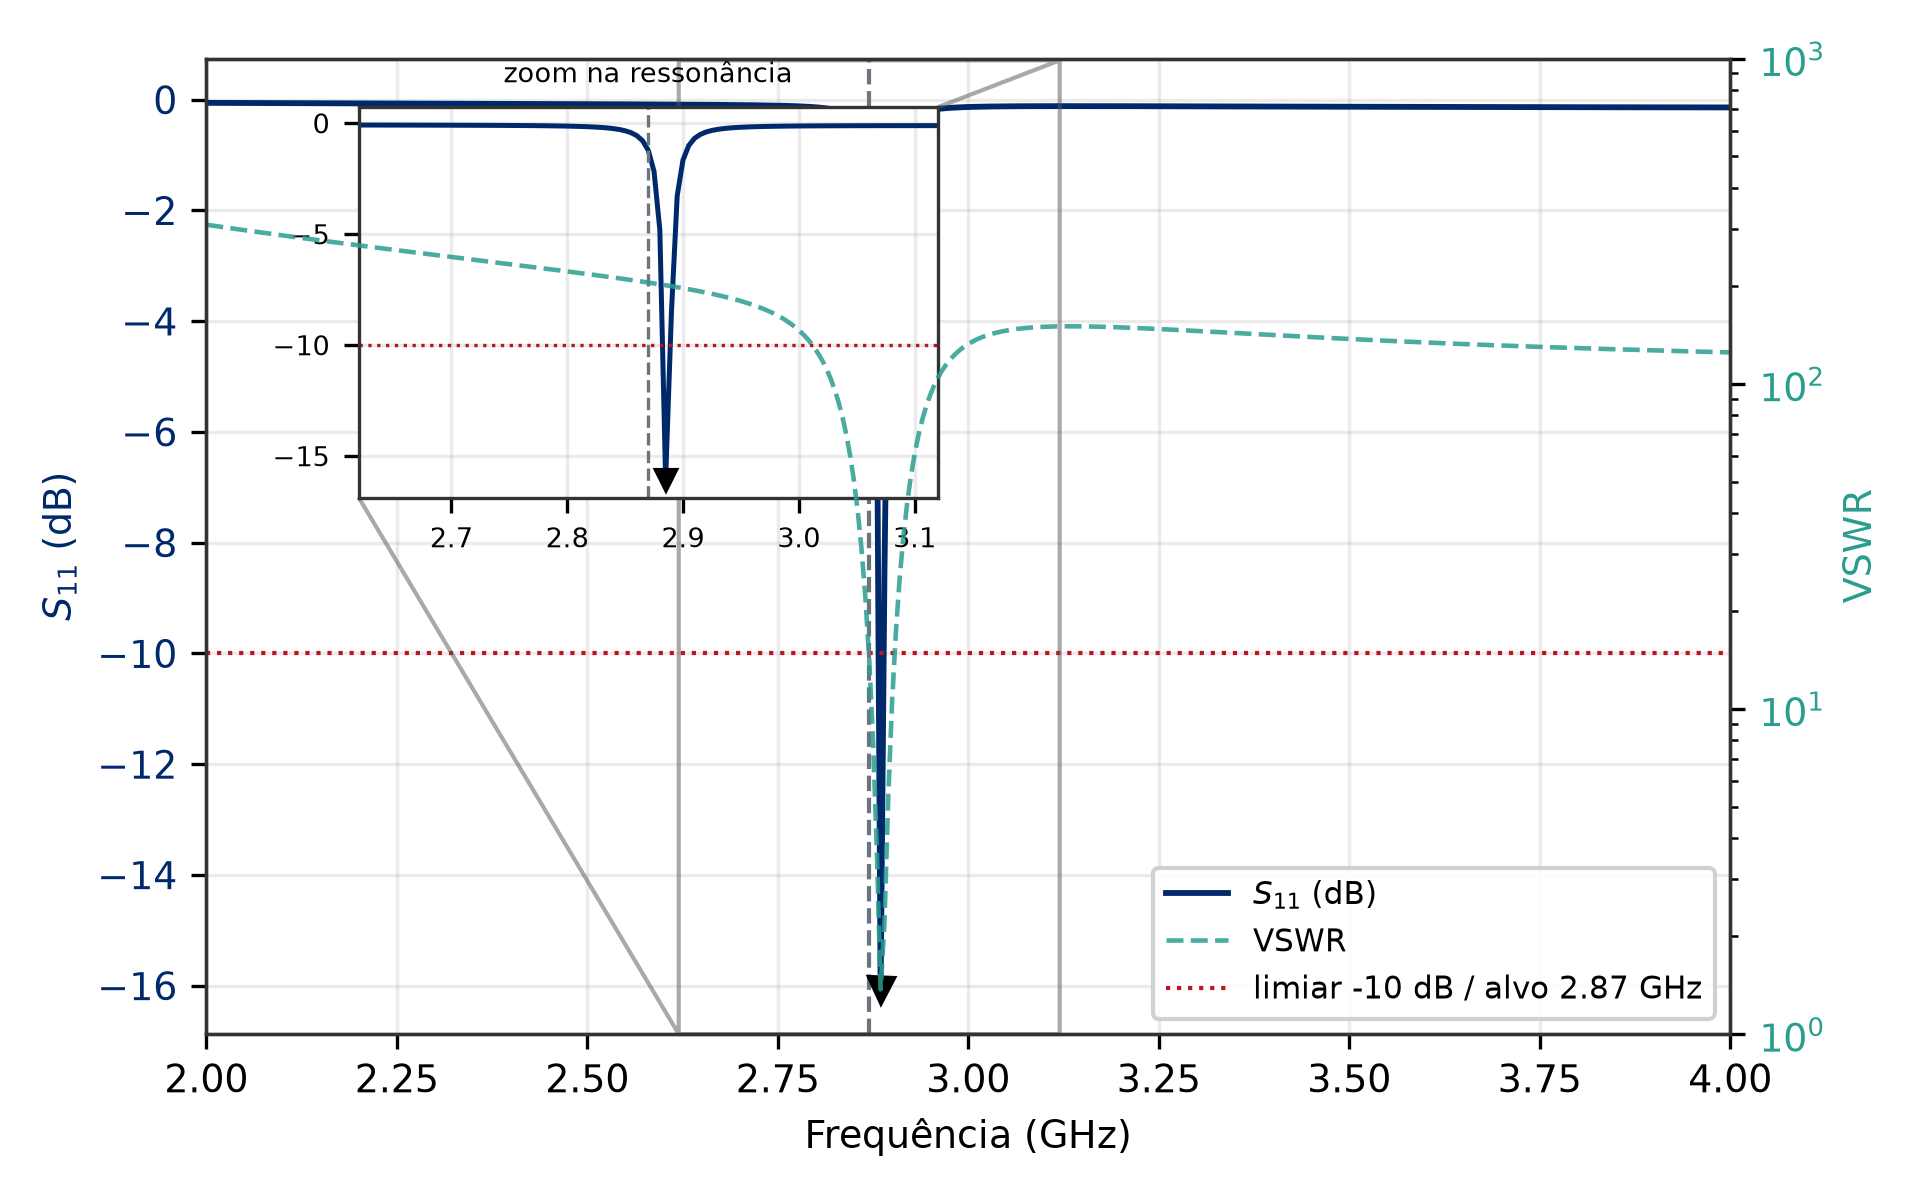
\includegraphics[width=0.82\textwidth]{../../aedt_project/datasheet_figs/fig_s11_vswr.png}\\[2pt]
\footnotesize Figura 4 -- $S_{11}$ (eixo esquerdo) e VSWR (eixo direito,
escala log) vs.\ frequ\^encia, 2--4\,GHz, com detalhe (\emph{inset}) da
regi\~ao de resson\^ancia. Linha vertical cinza: 2,87\,GHz (alvo NV$^-$).
Linha vermelha pontilhada: limiar de $-10$\,dB.
\end{center}

\vspace{4pt}
\textbf{Achado relevante:} o m\'inimo real de $S_{11}$ ocorre em
$f_0=2{,}885$\,GHz ($-16{,}1$\,dB), mas exatamente no ponto que importa
para a aplica\c{c}\~ao -- 2,87\,GHz -- o casamento cai para apenas
$-1{,}22$\,dB (VSWR~$\approx14{,}2$). O ressonador est\'a desalinhado do
alvo em $\approx15$\,MHz; um ajuste fino de $a_{spiral}$/$g_{cpl}$
desloca $f_0$ para coincidir com 2,87\,GHz.
\end{panel}

\clearpage

\begin{panel}{5. ARTES DE FABRICA\c{C}\~AO -- CORROSÃO COM PERCLORETO/CLORETO DE FERRO}
\begin{minipage}{0.42\textwidth}
\centering
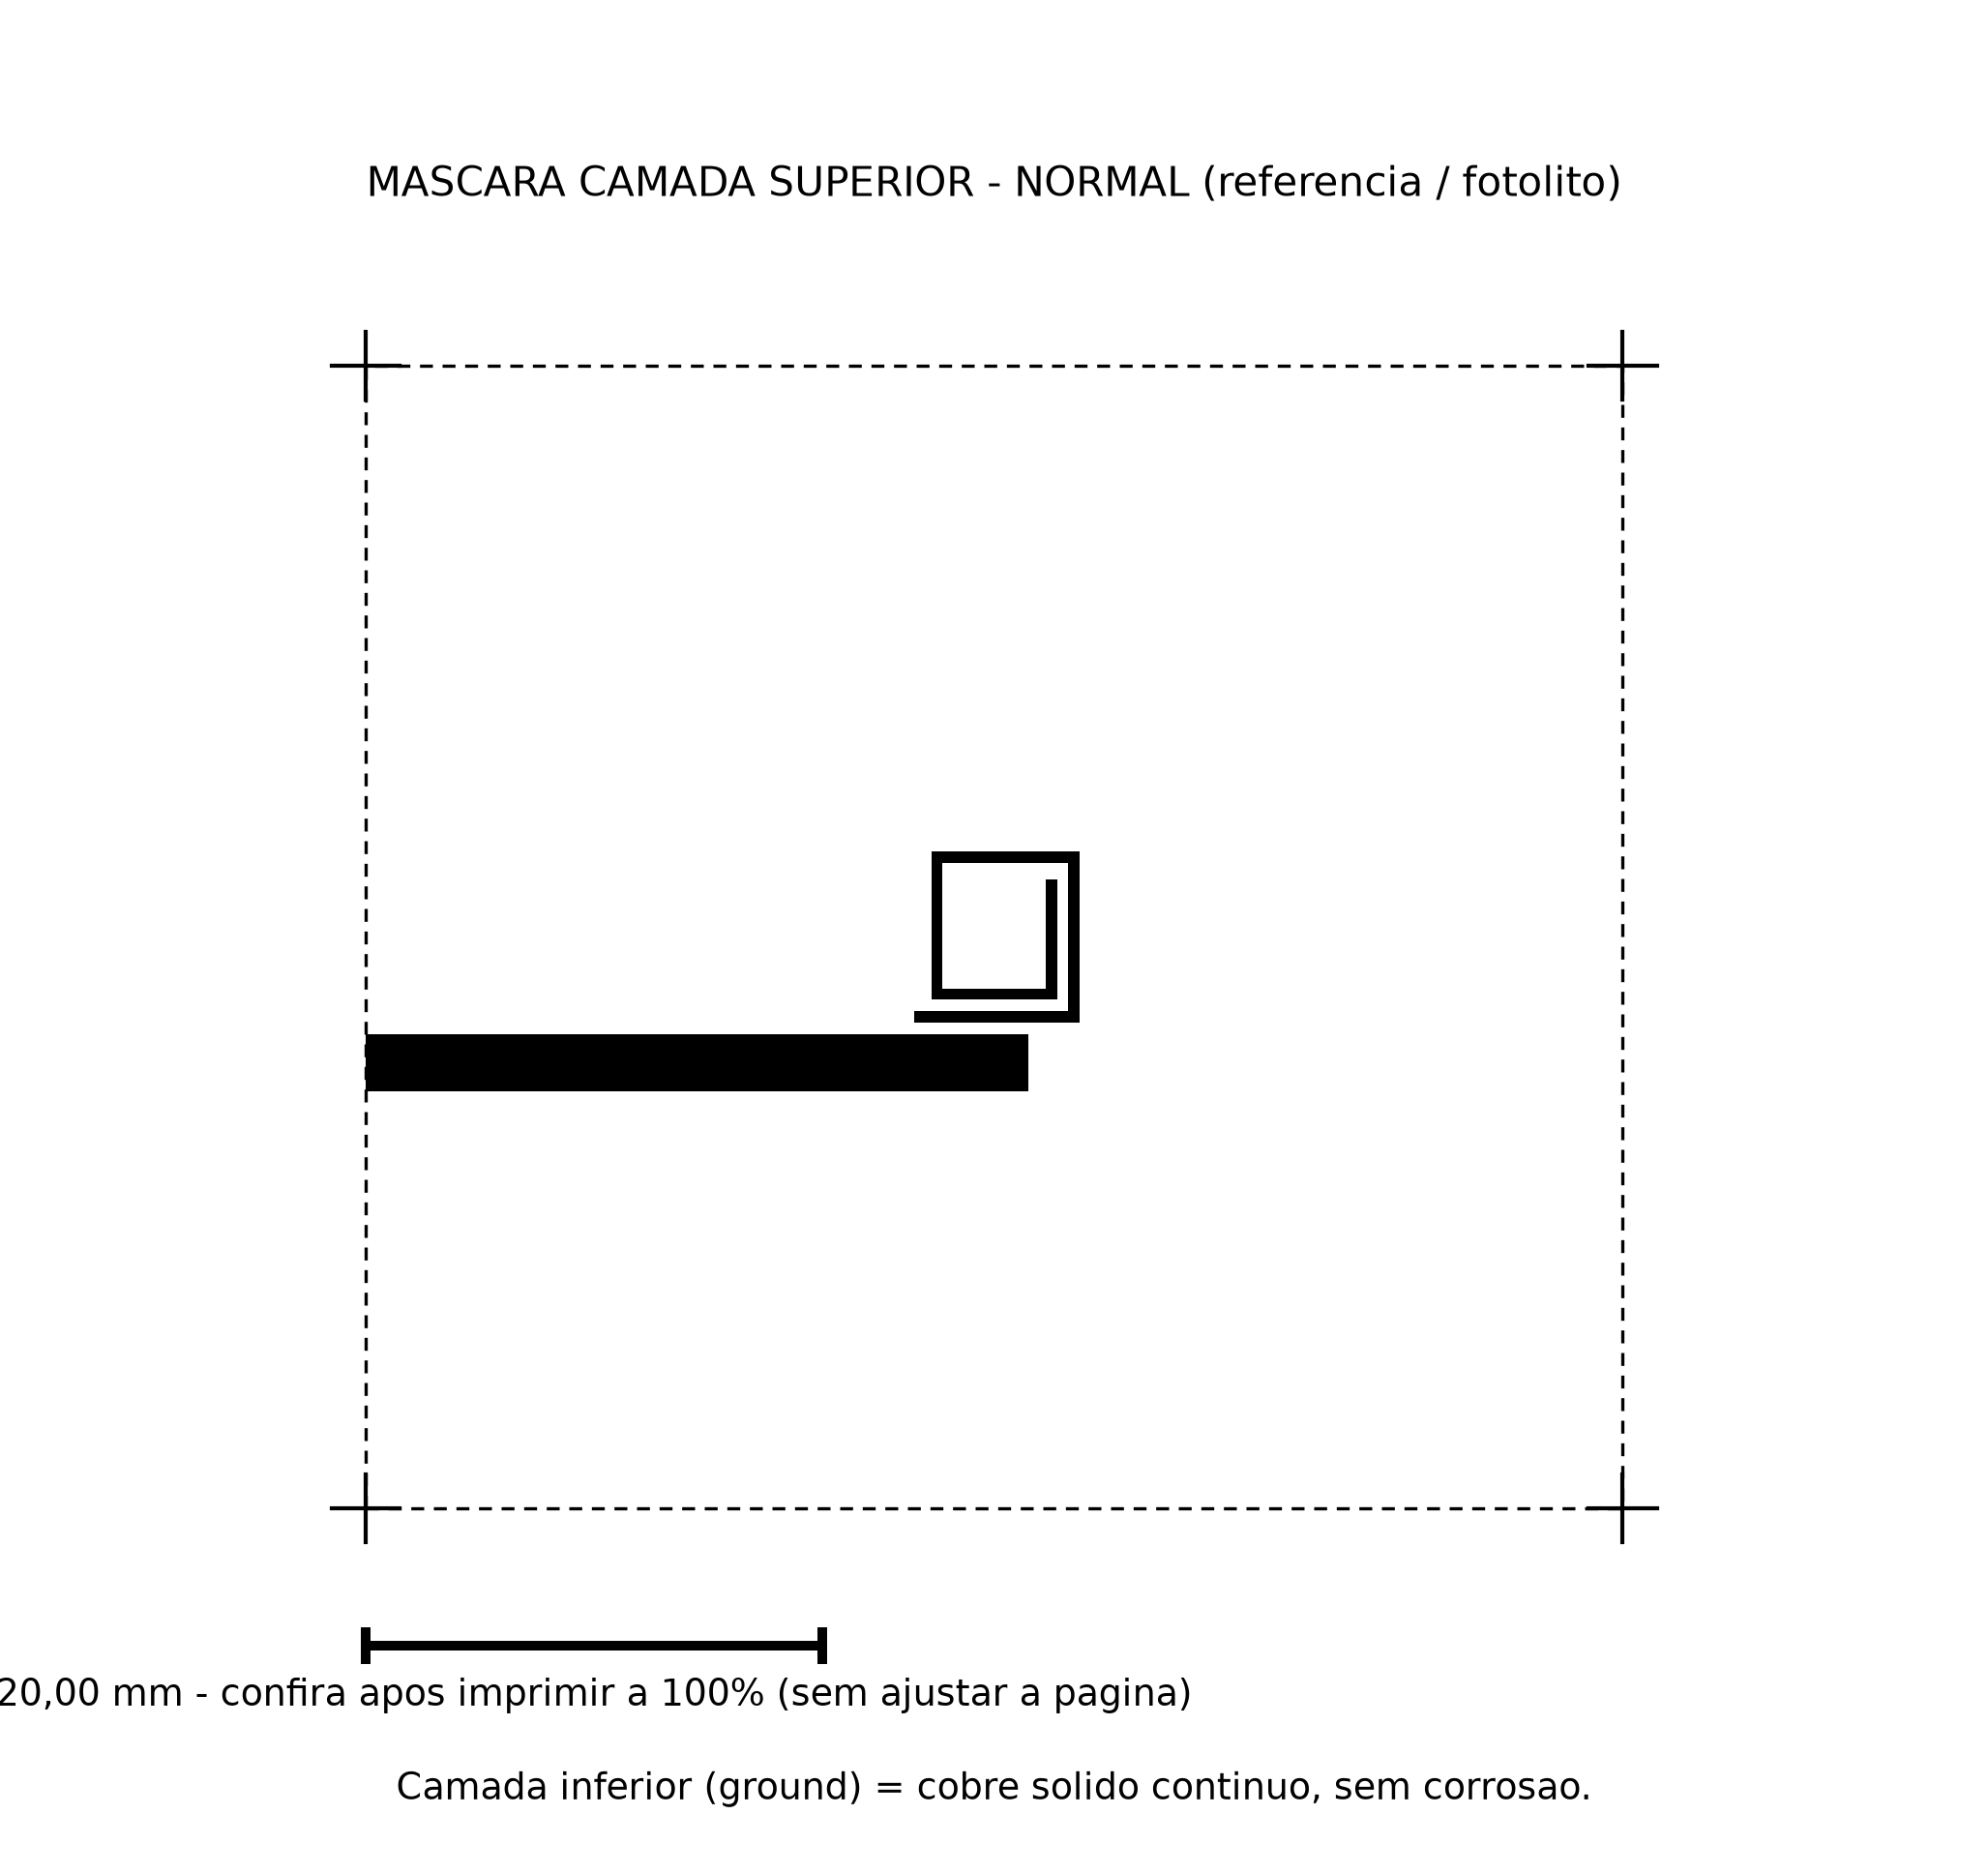
\includegraphics[width=\textwidth]{../../aedt_project/fabrication/mask_top_normal.png}\\[2pt]
\footnotesize Figura 5 -- Máscara da camada superior (pr\'e-visualiza\c{c}\~ao;
os arquivos completos est\~ao em escala real 1:1).
\end{minipage}%
\hfill
\begin{minipage}{0.54\textwidth}
\textbf{Arquivos prontos para impress\~ao} (pasta
\texttt{aedt\_project/fabrication/}):
\begin{itemize}[leftmargin=14pt, itemsep=2pt, topsep=2pt]
  \item \texttt{mask\_top\_normal.pdf/png} -- máscara como desenhada,
        para confer\^encia ou fotolito
  \item \texttt{mask\_top\_mirrored.pdf/png} -- máscara espelhada em X,
        necess\'aria no m\'etodo de transfer\^encia a ferro de passar
        (toner de impressora laser volta-se para o cobre)
\end{itemize}
\textbf{Procedimento recomendado:}
\begin{enumerate}[leftmargin=14pt, itemsep=1pt, topsep=2pt]
  \item Imprimir a máscara \emph{mirrored} em papel adequado para
        transfer\^encia (ou fotolito), sempre em escala \textbf{100\,\%
        / tamanho real} -- nunca "ajustar \`a p\'agina"
  \item Conferir a barra de calibra\c{c}\~ao de 20,00\,mm impressa na
        margem antes de transferir
  \item Cortar o substrato virgem em 55,0~$\times$~50,0\,mm (marcas de
        registro nos 4 cantos da máscara auxiliam o alinhamento)
  \item Transferir o t\^oner ao cobre (ferro de passar) e corroer em
        percloreto/cloreto de ferro
  \item A face inferior (\emph{ground}) \'e cobre s\'olido cont\'inuo --
        \textbf{n\~ao corroer}, manter integralmente met\'alizada
\end{enumerate}
\end{minipage}
\end{panel}

% ====================================================================
% PÁGINAS DE FABRICAÇÃO - MÁSCARAS PARA IMPRESSÃO EM PAPEL TRANSFER
% ====================================================================
\clearpage

\begin{panel}{6. M\'ASCARA NORMAL -- CAMADA SUPERIOR (CONFER\^ENCIA / FOTOLITO)}

\vspace{4pt}
\begin{center}
\fbox{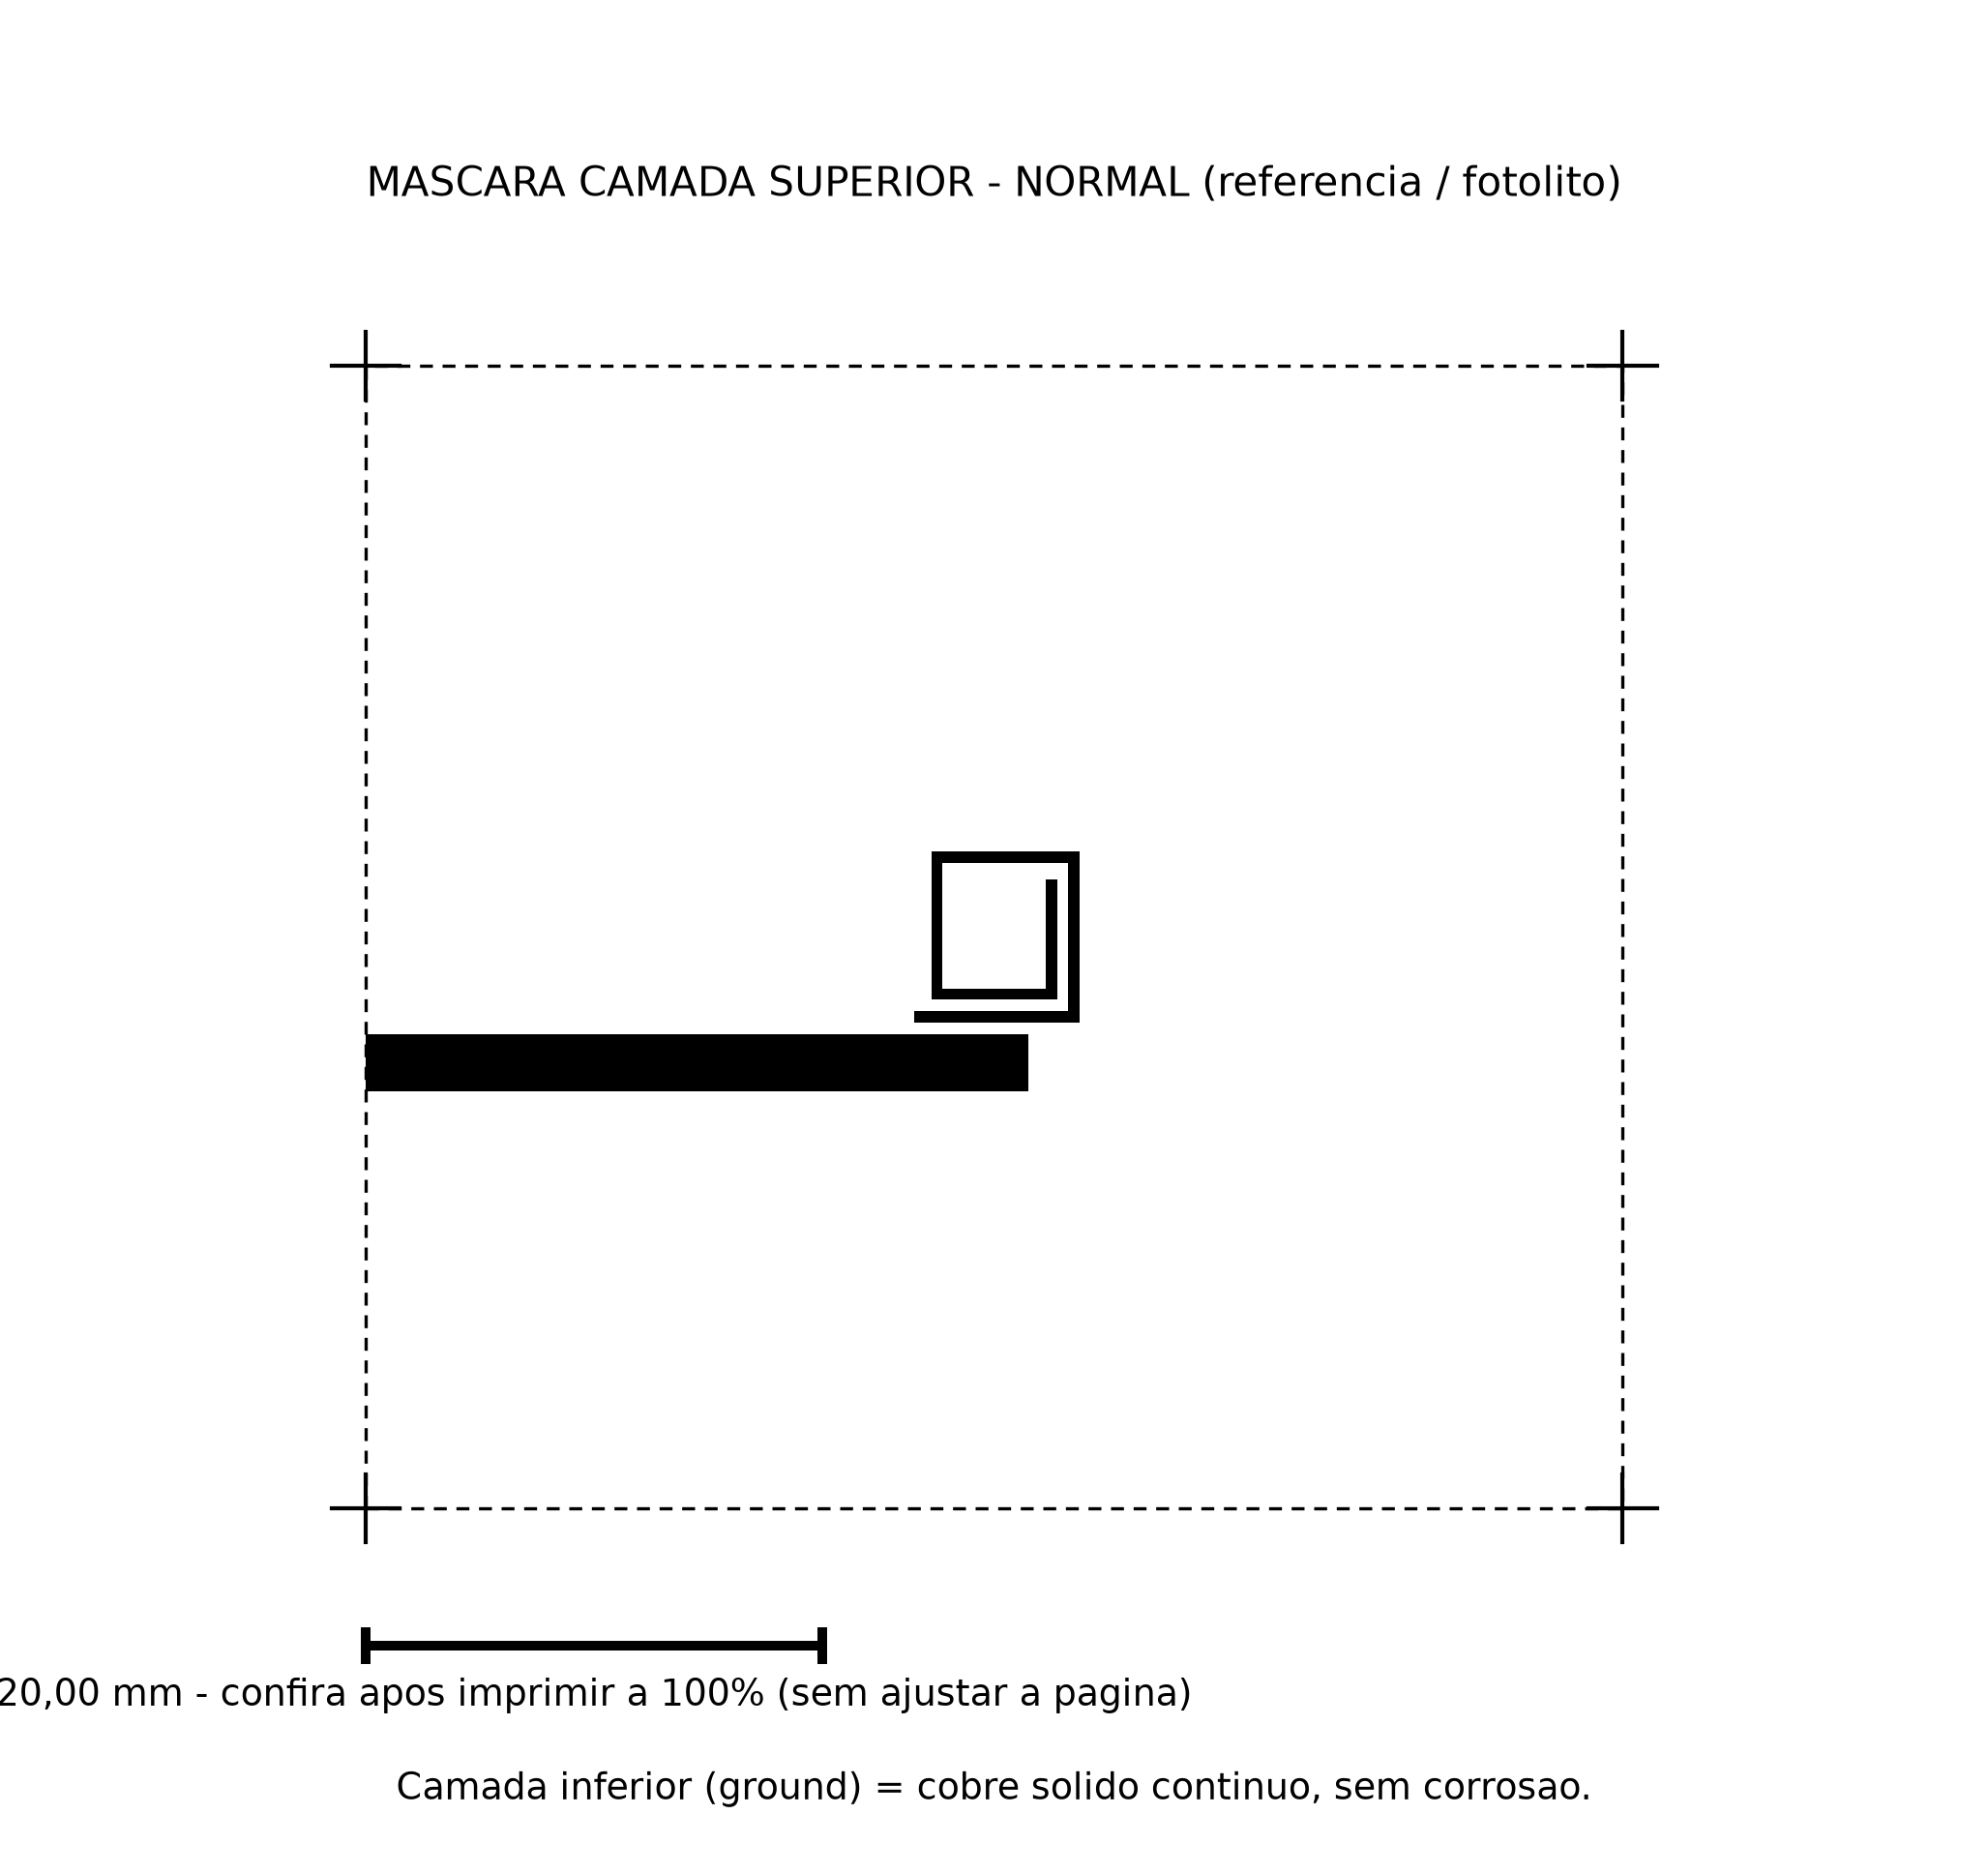
\includegraphics[width=0.85\textwidth]{../../aedt_project/fabrication/mask_top_normal.png}}
\end{center}
\vspace{4pt}

\footnotesize
\textbf{INSTRU\c{C}\~OES:} Esta p\'agina cont\'em a m\'ascara da camada
de cobre superior \textbf{como desenhada} (n\~ao espelhada). Use esta
p\'agina para:
\begin{itemize}[leftmargin=14pt, itemsep=1pt, topsep=1pt]
  \item Confer\^encia visual da geometria antes da fabrica\c{c}\~ao
  \item Fotolito (processo fotolitogr\'afico com filme fotossens\'ivel)
  \item Verifica\c{c}\~ao dimensional com paqu\'imetro ou r\'egua de
        precis\~ao sobre a barra de calibra\c{c}\~ao
\end{itemize}
\textcolor{alertred}{\textbf{ATEN\c{C}\~AO:}} Para o m\'etodo de
transfer\^encia t\'ermica (ferro de passar), use a m\'ascara
\textbf{espelhada} da p\'agina seguinte.

\normalsize
\end{panel}

\clearpage

\begin{panel}{7. M\'ASCARA ESPELHADA -- PARA TRANSFER\^ENCIA T\'ERMICA (FERRO DE PASSAR)}

\vspace{4pt}
\begin{center}
\fbox{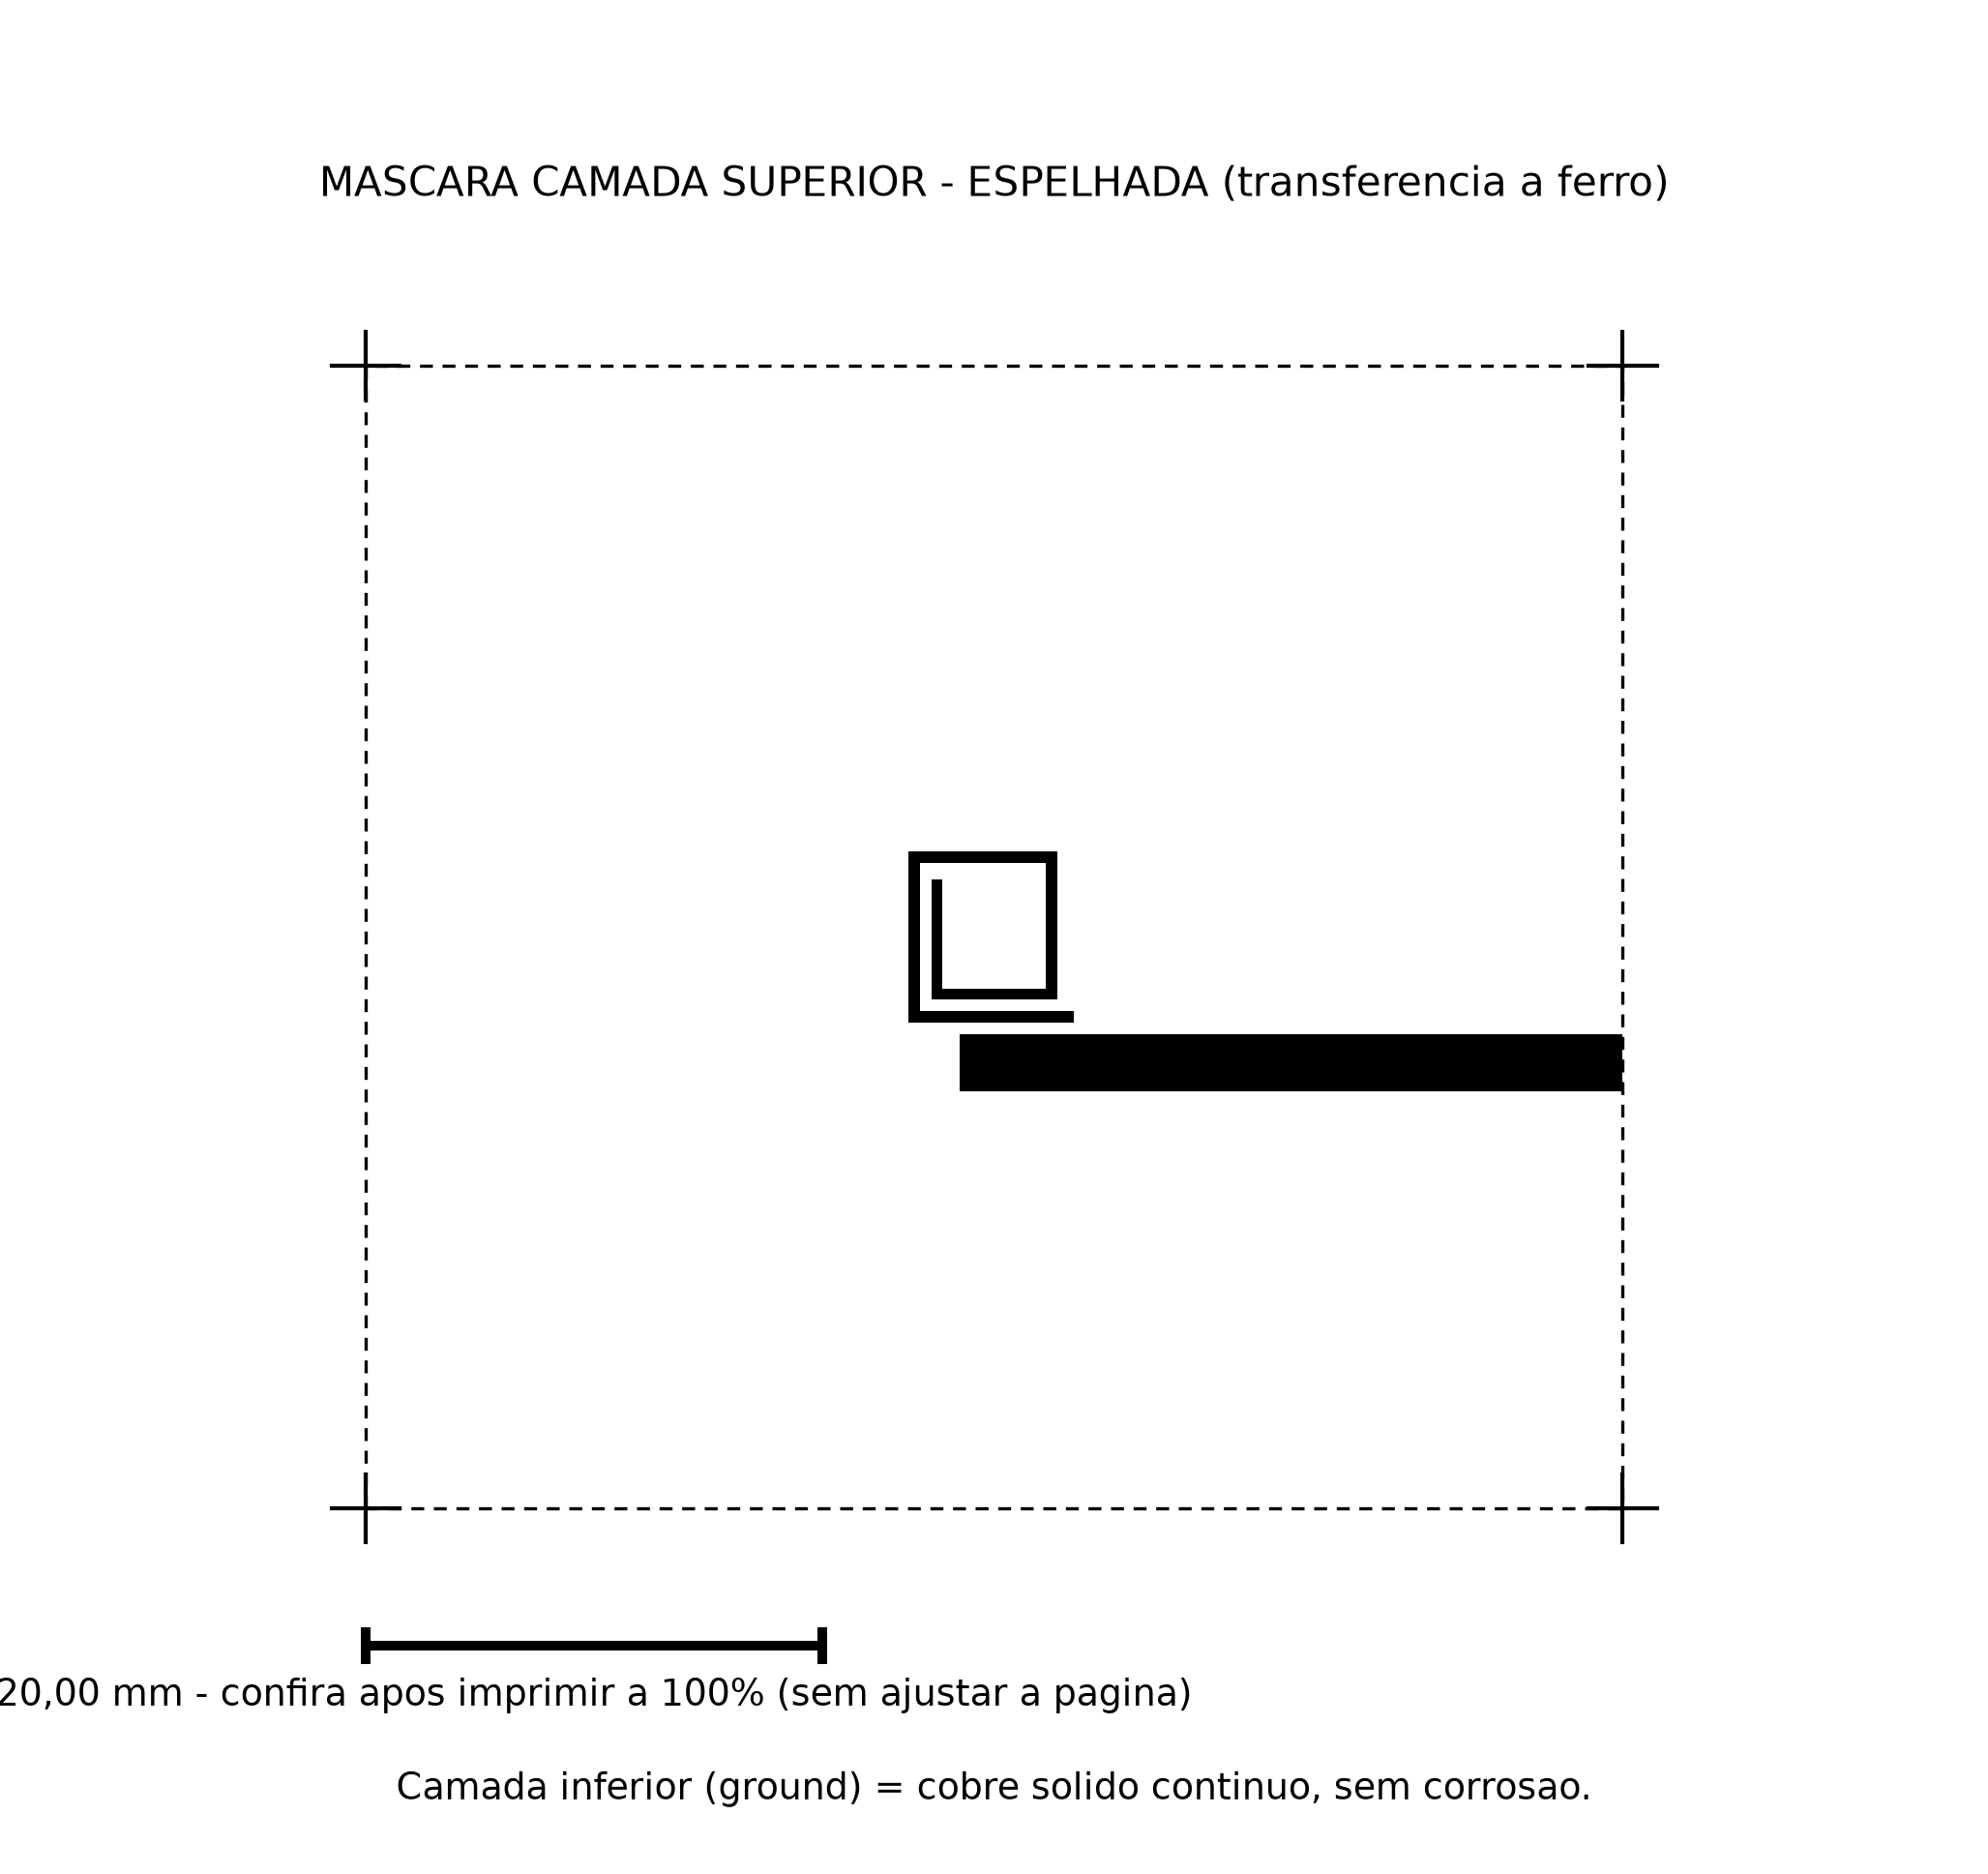
\includegraphics[width=0.85\textwidth]{../../aedt_project/fabrication/mask_top_mirrored.png}}
\end{center}
\vspace{4pt}

\footnotesize
\textcolor{alertred}{\textbf{ESTA \'E A P\'AGINA PARA IMPRIMIR E
TRANSFERIR AO COBRE.}}

\vspace{4pt}
\textbf{PROCEDIMENTO PASSO A PASSO:}
\begin{enumerate}[leftmargin=14pt, itemsep=2pt, topsep=2pt]
  \item \textbf{Imprimir} esta p\'agina em \textbf{impressora laser}
        (nunca jato de tinta) sobre papel \emph{glossy} (papel
        fotogr\'afico ou transfer espec\'ifico para PCB). Configurar a
        impressora para \textbf{100\,\% / tamanho real} -- desativar
        qualquer op\c{c}\~ao de ``ajustar \`a p\'agina'' ou ``redimensionar''
  \item \textbf{Verificar escala:} medir a barra de calibra\c{c}\~ao
        de 20,00\,mm impressa na margem com paqu\'imetro. Se a medida
        diferir mais de 0,1\,mm, reconfigurar e reimprimir
  \item \textbf{Preparar o substrato:} cortar o Rogers RO5880 virgem
        em 55,0~$\times$~50,0\,mm. Limpar a face de cobre com
        palha de a\c{c}o fina (\#0000) e \'alcool isoprop\'ilico
  \item \textbf{Posicionar:} colocar a face impressa (t\^oner) voltada
        para baixo, diretamente sobre o cobre limpo. Alinhar usando as
        marcas de registro nos 4 cantos
  \item \textbf{Transferir:} aplicar ferro de passar (temperatura
        m\'axima, sem vapor) com press\~ao firme e uniforme por
        3--5 minutos. Mover o ferro lentamente cobrindo toda a \'area
  \item \textbf{Resfriar e remover papel:} mergulhar em \'água morna
        por 5--10 min, depois descolar o papel cuidadosamente.
        Retocar falhas com caneta permanente resistente a \'acido
  \item \textbf{Corroer:} imergir em solu\c{c}\~ao de percloreto de
        ferro (FeCl$_3$) ou cloreto de ferro (FeCl$_2$) a
        $\approx40\,{}^\circ$C, agitando periodicamente, at\'e remover
        todo o cobre exposto (tipicamente 10--30 min)
  \item \textbf{Limpar:} remover o t\^oner residual com acetona ou
        thinner. Lavar com \'água e secar
  \item \textbf{Face inferior (ground):} \textbf{N\~AO CORROER} --
        manter o cobre s\'olido cont\'inuo integralmente met\'alizado
\end{enumerate}

\vspace{4pt}
\textbf{Dimens\~oes do substrato:}
55,0~$\times$~50,0\,mm, espessura 0,75\,mm, cobre 1\,oz (35\,$\mu$m)
ambos os lados.

\normalsize
\end{panel}

\vfill
\begin{center}
\footnotesize\color{steel}
\textbf{Autores:} Jo\~ao Victor Vieira Faria \quad$\vert$\quad Thiago Ferreira
\quad$\vert$\quad \textbf{Orientador:} Prof.\ Dr.\ Achiles Fontana da Mota\\[1pt]
Universidade de Bras\'ilia (UnB) -- Departamento de Engenharia El\'etrica (ENE)
-- Faculdade de Tecnologia
\end{center}

\end{document}